\subsubsection{Costo temporal}

El algoritmo KNN es temporalmente costoso ya que para calcular la distancia entre dos vectores hay que considerar a todas sus coordenadas. Por lo tanto somos muy dependientes del tamaño del vector, que en general al trabajar con imágenes suelen ser bastante grandes.


Para analizar nuestro dataset con KNN utilizamos cross validation con $K = 5$ y $K = 10$.

En la siguiente figura se pueden ver los tiempos de ejecución promedio de las particiones para cada valor de K.

\begin{figure}[h!]
  \begin{center}
	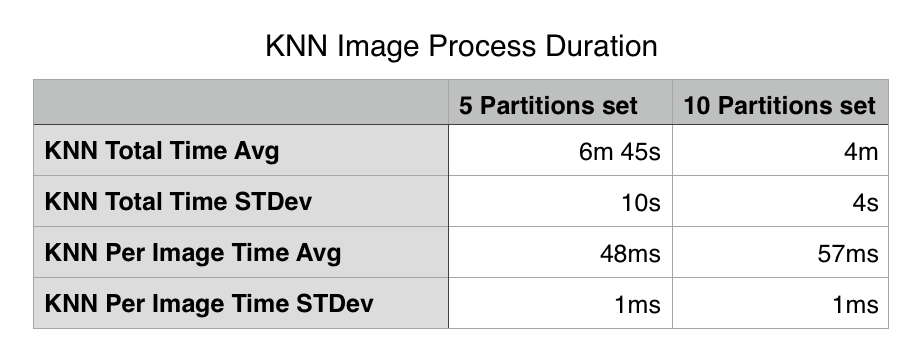
\includegraphics[scale=0.7]{exp1/KNN-Image-Process-Duration.png}
	\caption{KNN Image Process Duration}
%	\label{accum_var_PCA}
  \end{center}
\end{figure}


Para el caso de $K = 5$ obtuvimos que etiquetar una imagen usando KNN tardó en promedio 48ms, que aunque parece poco, al correr todo nuestro set de test de 8400 imágenes se obtuvo un tiempo de ejecución promedio de 6.75 minutos con 10 segundos de desvío estándar. Se puede observar fácilmente que si quisiésemos clasificar un millón de imágenes se tardaría aproximadamente 13 horas.

Por otro lado, vemos que si realizamos 10 particiones a nuestro dataset, el tiempo de procesamiento de cada imagen aumenta de 48ms a 57ms. Esto se debe a que con 10 particiones se debe buscar el vecino más cercano entre más imágenes.

Debemos aclarar también que el costo temporal de variar la cantidad de vecinos de KNN es lineal y por lo tanto esto no tiene una influencia significativa en el tiempo de ejecución. En consecuencia decidimos analizar la calidad de los resultados de KNN disminuyendo la importancia del costo de agregar más vecinos.

\subsubsection{Calidad del algoritmo}

Analizamos la calidad de KNN (con K = 5) calculando su Hit Rate, Precision, Recall y F1 score. Se pueden observar los resultados en el siguiente gráfico.

\newpage

\begin{figure}[h!]
  \begin{center}
	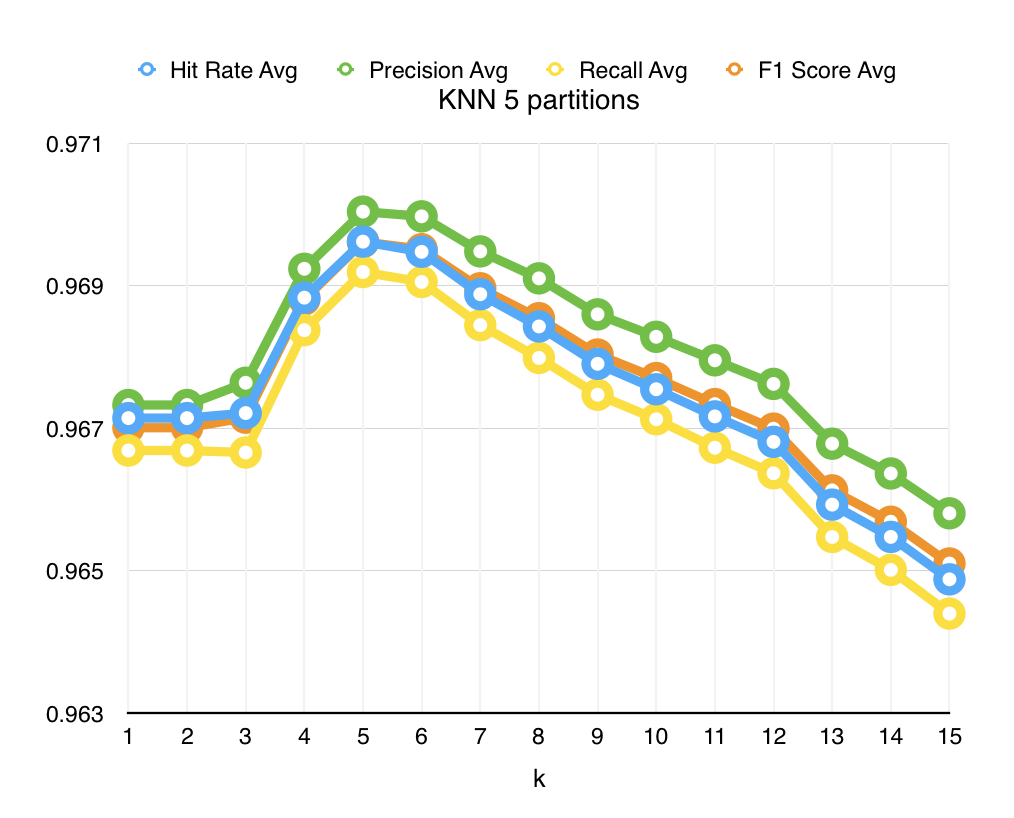
\includegraphics[scale=0.7]{exp1/KNN-5p-Scores.png}
	\caption{KNN quality comparison}
%	\label{accum_var_PCA}
  \end{center}
\end{figure}

Una de las primeras cosas que se pueden observar es que la calidad de los resultados es extremadamente buena. El hit rate promedio para el mejor k es 0.97.

\textcolor{red}{Explicar Precision, Recall y F1}\\

Por otro lado también se puede ver que, a partir de k = 5, al aumentar la cantidad de vecinos la calidad de los resultados disminuye. Esto se debe probablemente a que considerar más imágenes comienza a agregar ruido a la medición. Al considerar más vecinos que cada vez se empiezan a parecer menos, es posible que se incorporen un conjunto cada vez mayor de imágenes que pertenecen a otra clase. Así mismo podemos ver que desde 1 vecino hasta 5 la información que aporta agregar más vecinos es valiosa y ayuda mejorar la clasificación.\\

Analizando el hit rate más detalladamente obtenemos el siguiente gráfico donde podemos observar su desvío estándar.

\newpage

\begin{figure}[h!]
  \begin{center}
	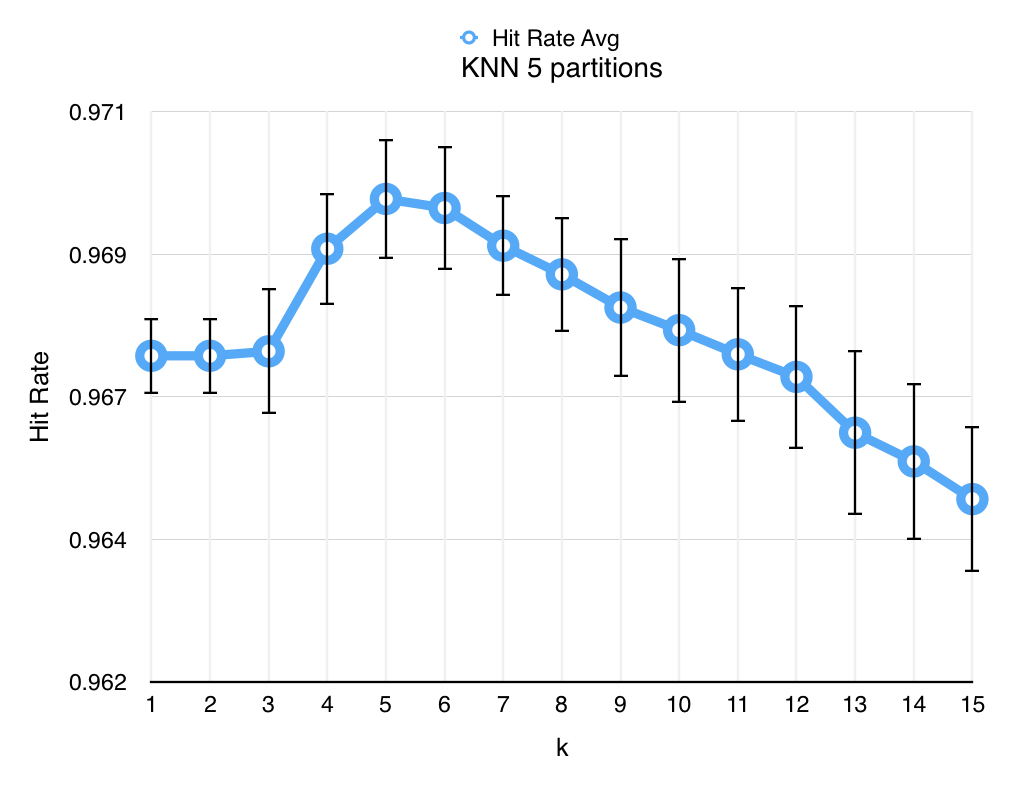
\includegraphics[scale=0.7]{exp1/KNN-5p-Hit-Rate.png}
	\caption{KNN hit rate}
%	\label{accum_var_PCA}
  \end{center}
\end{figure}

Por un lado podemos ver que el desvío estándar es relativamente pequeño. Este desvío representa los diferentes resultados del Hit Rate para cada partición de nuestro data set. Entonces sabemos que todas nuestras particiones tienen un buen resultado y no estamos sesgando nuestro testeo.
Otra cosa interesante que se desprende del gráfico es que los desvíos estándar van aumentando a medida que se incrementa la cantidad de vecinos de KNN. De hecho en el siguiente gráfico podemos ver este incremento.

\begin{figure}[h!]
  \begin{center}
	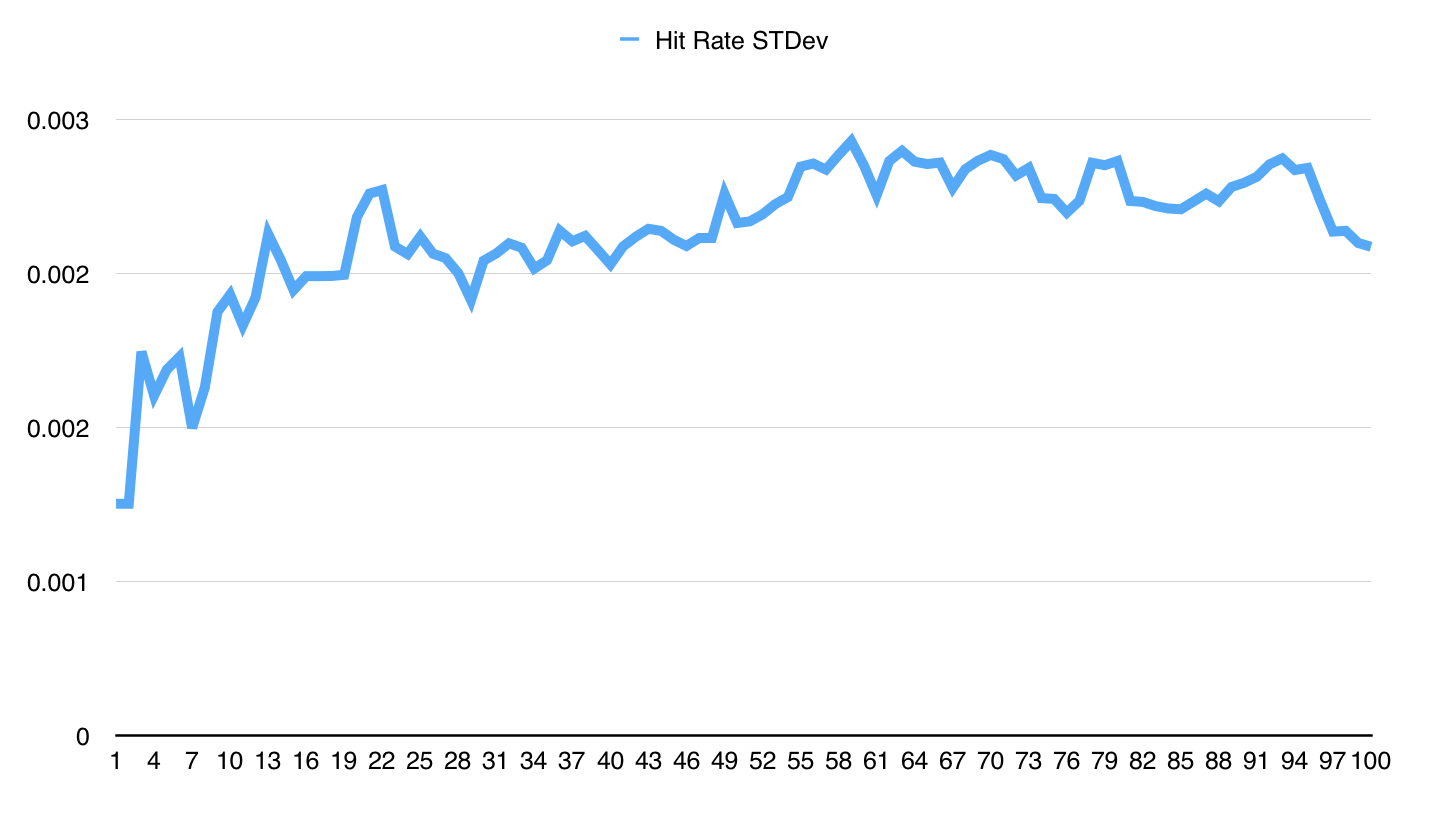
\includegraphics[scale=0.5]{exp1/KNN-5p-Hit-Rate-stdev.png}
	\caption{KNN hit rate standard deviation}
%	\label{accum_var_PCA}
  \end{center}
\end{figure}

Aunque los números se mantienen pequeños, es claro que agregar más vecinos incrementa el ruido y hace divergir más la calidad de los resultados en cada partición.\\

Una vez determinado que k = 5 optimiza la calidad de KNN y además no compromete el tiempo de ejecución, veamos en particular cómo está clasificando a nuestro dataset.


\begin{figure}[h!]
  \begin{center}
	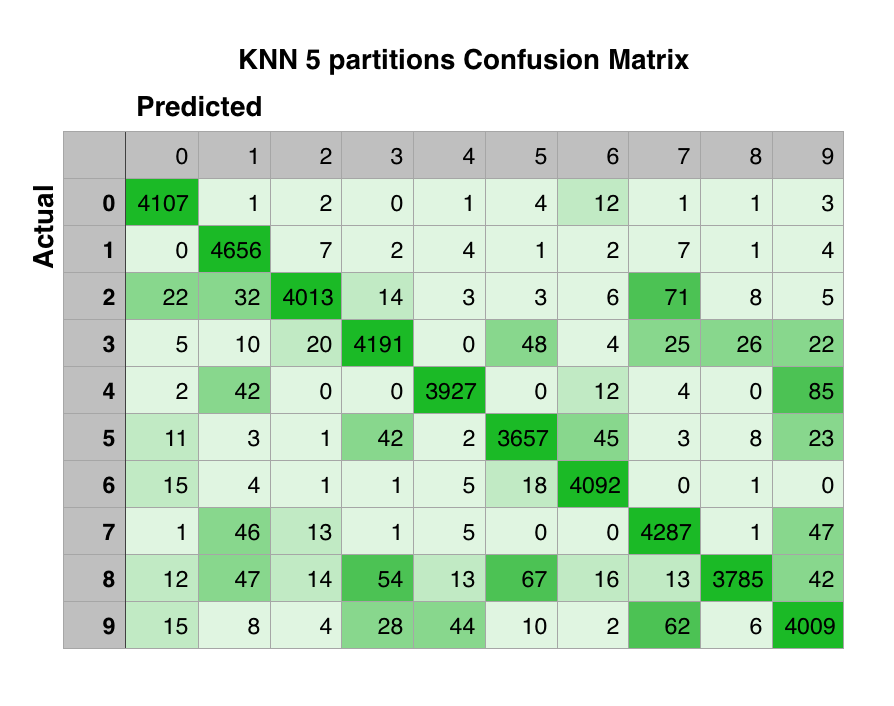
\includegraphics[scale=0.7]{exp1/KNN-5p-Confusion.png}
	\caption{KNN Confusion Matrix}
%	\label{accum_var_PCA}
  \end{center}
\end{figure}

Esta matriz de confusión es la suma de las matrices de confusión de cada una de las 5 particiones del test. Nos muestra claramente en su diagonal las clasificaciones acertadas y en el resto de las posiciones las que no clasificó correctamente. Vemos que los números fuera de la diagonal en general son bajos y que los más altos en general son casos que justifican cierto error. Por ejemplo, hubo setenta y un $2$ que clasificó como $7$ y a su vez hubo cuarenta y seis $7$ que clasificó como $2$. También vemos cierta confusión entre el 4 y 9, 8 y 5, etc.\\ 


Todo este análisis realizado para K = 5 lo hicimos también para K = 10. 

En el siguiente gráfico podemos observar que las medidas de calidad son similares al anterior caso y k = 5 sigue siendo el máximo.\\

\newpage

\begin{figure}[h!]
  \begin{center}
	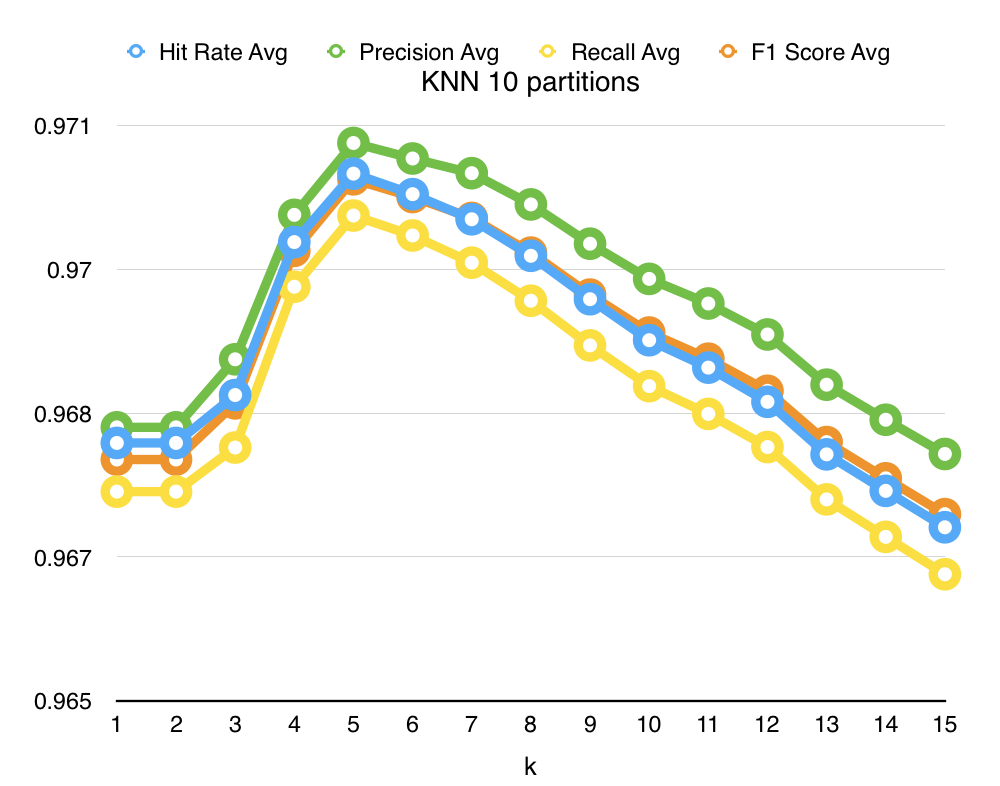
\includegraphics[scale=0.7]{exp1/KNN-10p-Scores.png}
	\caption{KNN Hit Rate (10 partitions)}
%	\label{accum_var_PCA}
  \end{center}
\end{figure}

Comparando los desvíos estándar se puede ver que con 10 particiones el desvío es bastante superior al caso anterior. Esto probablemente se deba a que al haber más particiones de tamaño más pequeño, los casos que la base de entrenamiento no sabe reconocer no estén tan uniformemente distribuidos en esos 10 conjuntos.\\ 

\begin{figure}[h!]
  \begin{center}
	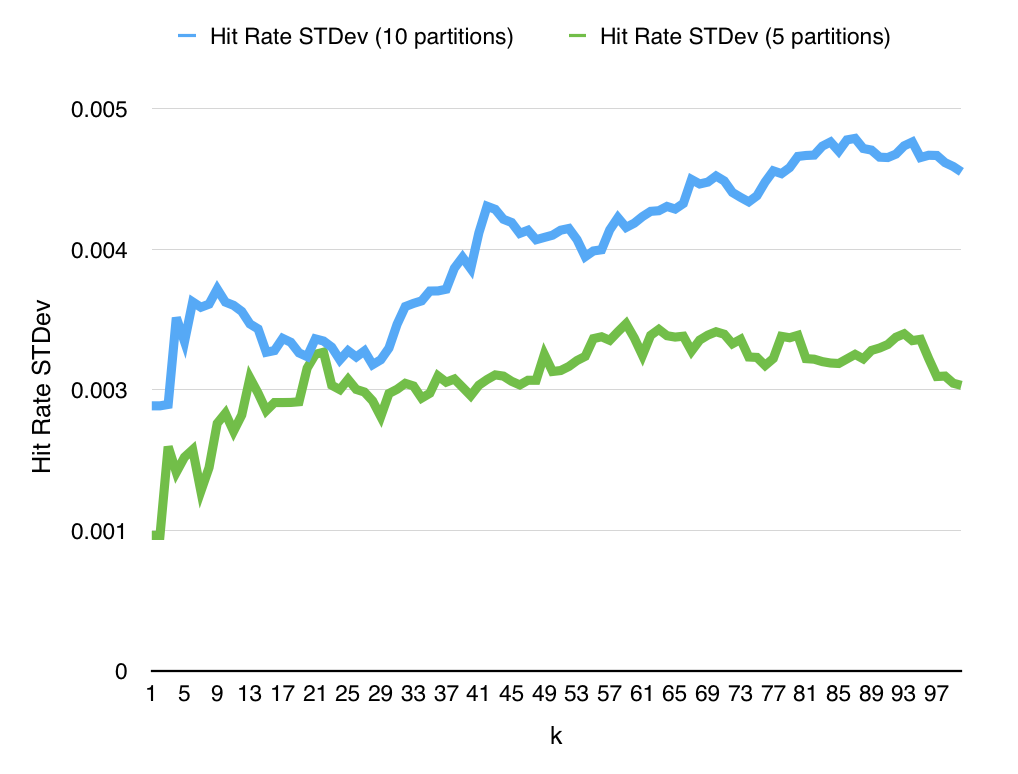
\includegraphics[scale=0.7]{exp1/KNN-Hit-Rate-stdev.png}
	\caption{KNN Hit Rate (10 partitions)}
%	\label{accum_var_PCA}
  \end{center}
\end{figure}

Por último comparamos el hit rate entre los 2 conjuntos de particiones y observamos que el caso de 10 particiones tiene un hit rate ligeramente superior. Esto se debe a que su base de entrenamiento es más grande y puede así reconocer mejor los dígitos.\\

\begin{figure}[h!]
  \begin{center}
	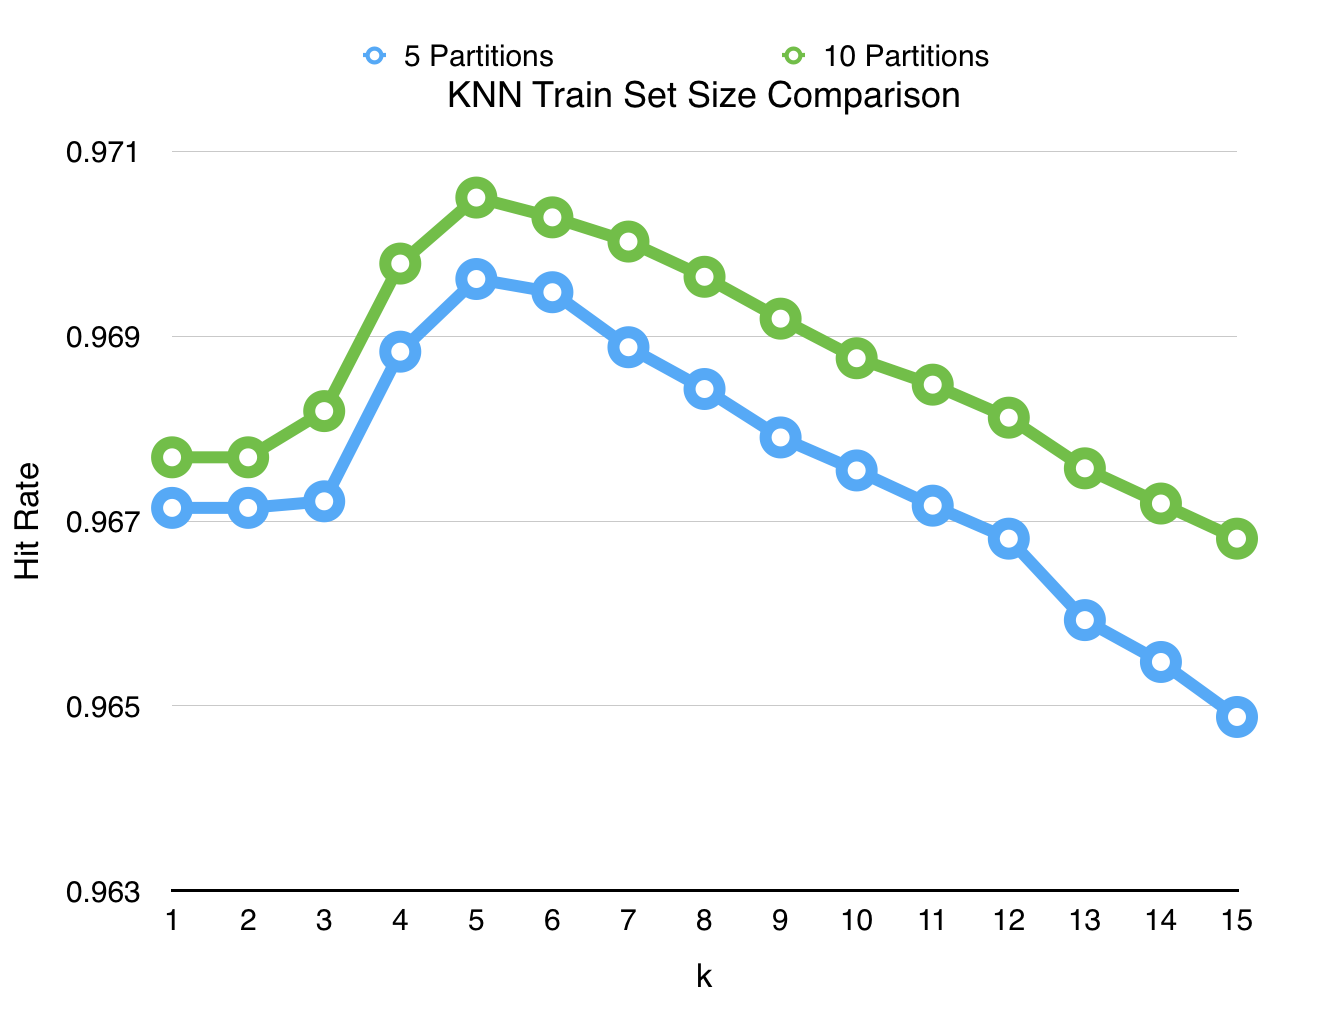
\includegraphics[scale=0.6]{exp1/KNN-Train-Set-Size.png}
	\caption{KNN Hit Rate (10 partitions)}
%	\label{accum_var_PCA}
  \end{center}
\end{figure}



